\mychapter{Successions i progressions}{Successions i progressions}{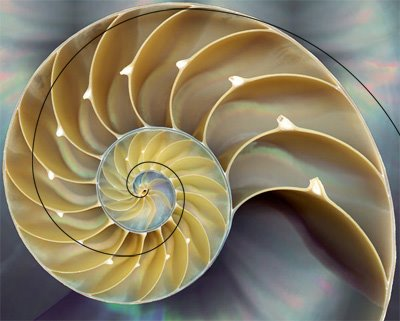
\includegraphics[width=4.3cm]{img-03/nautilus}}{chap:successions}


\vspace*{\fill}


\begin{iniaval}
 \textbf{Esbrina la regla que s'ha emprat i escriu tres nombres més de les llistes següents:}

\begin{tasks}
	\task  1, 3, 5, 7, .... , .... , ....,  $\cdots$
	\task  2, -4, 8, -16, 32, .... , .... , ....,  $\cdots$
	\task  1, 4, 9, 16, 25, 36, .... , .... , ....,  $\cdots$
\end{tasks}

\vspace{0.25cm}
\quad Inventa't una llista semblant i passa-la al teu company perquè endevini els següents termes.
\vspace{0.25cm}

 \textbf{Col·loca les paraules i forma la frase}
\vspace{0.5cm}
\begin{center}
 \textbf{REGLA \qquad\qquad LLISTA  \qquad\qquad  SUCCESSIÓ  \qquad\qquad  FIXADA  \qquad\qquad NOMBRES}
\end{center}
\vspace{0.5cm}
 \textbf{``Una ................. és una .................ordenada de .................obtinguts a partir d'una .................de formació ................''}

\vso
 
\addanswersline[cols=1]{Avaluació inicial}{0}{[Successió dels nombres senars: $1,3,5,7,9,11,13,15,\cdots$, Multiplicam per --2:\par $2,-4,8,-16,32,-64,128,-256,\cdots$, Successió dels quadrats:\par $1,4,9,16,25,36,49,64,81,\cdots$ ]}
\end{iniaval}

\vspace*{\fill}

\pagebreak
\section{ Successions}

\begin{theorybox}
 \video[ytid=MUZZ7aFAIDA]{134}{Successions}
 Una \textbf{successió} és una \textbf{llista ordenada} de nombres obtinguts a partir d'una regla de formació fixada. A cadascun dels nombres se'ls anomena \textbf{terme}. Per exemple, la llista de nombres senars 1, 3, 5, $\cdots$ té com a primer terme $a_1 = 1$, segon terme $a_2=3$, etc.
 
 Una successió es pot donar de diferents formes:
 \begin{itemize}
 	\exer Donants els seus primers termes: 1, 3, 5, 7, $\cdots$
 	\exer A partir del terme general:  $a_n = 2n-1$
 	\exer A partir d'una relació de recurrència:  $a_1 = 1$ i $a_{n+1} = a_n + 2$
 \end{itemize}
\end{theorybox}
\vspace{-0.5cm}
\begin{blueshaded}
	Una manera forma fàcil d'entendre què és una successió és agafar la llista de classe i escriure devora de cada número de llista, per exemple, el mes de naixement de l'alumne:
	
	\begin{minipage}{0.5\textwidth}
	 	\begin{tabular}{lcc}
	 	\textbf{Nom} & $\mathbf{n}$ & $\mathbf{a_n}$ \\ \hline	
	 	\emph{Amengual} & 1 $\rightarrow$ & 2 \\
	 	\emph{Bibiloni} & 2 $\rightarrow$ & 7 \\
	 	\emph{Cerdà}    & 3 $\rightarrow$ & 5 \\
	 	\emph{Deyà}    & 4 $\rightarrow$ & 11
	 \end{tabular}
	\end{minipage}
	\begin{minipage}{0.5\textwidth}	
		En la successió $a_n= 2, 7, 5, 11, \cdots$,
		
		\qquad $\mathbf{a}$ és el valor del mes 
		 
		 \qquad $\mathbf{n}$ és el número de llista.
	\end{minipage}
\end{blueshaded}


\begin{mylist}

\exer  \spen Escriu els deu primers termes de les següents successions:
\begin{tasks}(3)
	\task   $-$1, $-$2, $-$3, $-$4,{\dots}   
	\task  1, 4, 9, 16,{\dots}   
	\task  1, 3, 5, 7,{\dots}
\end{tasks}
\vso
\answers[cols=1]{[$-1,-2,-3,-4,-5,-6,-7,-8,-9,\cdots$, $1,4,9,16,25,36,49,64,81,100,\cdots$, $1,3,5,7,9,11,13,15,17,\cdots$]}

\exer \spen  Escriu el terme que ocupa el lloc 100 de cadascuna de les successions anteriors.
\vso
\answers[cols=1]{[$a_n=-n;\,\,a_{100}=-100$, $a_n=n^2;\,\,a_{100}=100^2=10000$. $a_n=2n-1,\,\,a_{100}=199$]}

\exer  Sabem que un cos que cau lliurement sobre la Terra té una velocitat que augmenta 9,8 m/s cada segon. Si en el primer segon la seva velocitat és de 15 m/s, escriu en el teu quadern la velocitat en els segons indicats en la taula. Observes alguna regla que et permeti conèixer la velocitat al cap de 20 segons? Representa gràficament aquesta funció.
\end{mylist}
\begin{center}
\renewcommand{\arraystretch}{2}
\begin{tabular}{|p{0.25\textwidth}|p{0.2\textwidth}|p{0.2\textwidth}|p{0.2\textwidth}|}\hline 
\textbf{Temps en segons} & 1 & 2 & 3 \\ \hline 
\textbf{Velocitat en m/s} & 15 &  &  \\ \hline 
\end{tabular}
\end{center}

\answers{Les velocitats són passats $n$ segons  $v_n=15+(n-1)\cdot 9.8$.\par Passats $n=2$ segons; $v_2=24.8$ m/s. \par Passats $n=3$ segons; $v_3=34.6$ m/s. \par Passats $n=20$ segons; $v_{20}=15+(20-1)\cdot 9.8=201.2$ m/s.} 
 
\pagebreak
 
\begin{resolt}[E]{
		Troba els 5 primers termes de la successió donada en forma recurrent:
		
		$a_1 = 2$
		
		$a_2 = 1$
		
		$a_n = 3 a_{n-1} + 2 a_{n-2}$
		
	}
	Ens donen el primer i segon termes i la relació per trobar els següents. El tercer terme s'obté de fer el triple del segon més el doble del primer.
	\[ a_3 = 3 \cdot 1 + 2 \cdot 2 = 7  \]
	\[ a_4 = 3 \cdot 7 + 2 \cdot 1 = 23  \]
	\[ a_5 = 3 \cdot 23 + 2 \cdot 7 = 83  \]
	\[ \cdots \]
\end{resolt}

\begin{mylist}

\exer  Escriu els quatre primers termes de les següents successions: 

 $a_n = 2 n^2+1$  \quad \quad  $b_n = \frac{4n-1}{3n}$ \quad \quad
 %%%%
 $ \begin{array}{c}
c_1\ =\ 1; \\ 
c_n\ =\ 3c_{n-1}\ +\ 5 \end{array}
$
\quad \quad
%%%%
$\begin{array}{c}
d_1=\ 2;\ \ d_2=5; \\ 
d_n\ =\ 2d_{n-1}\ +\ d_{n-2} \end{array}$
 
 \answers[cols=1]{[$a_n=3,9,19,33,\cdots$, $b_n=1,\frac{7}{6},\frac{11}{9},\frac{5}{4},\cdots$, $c_n=1,8,29,92,\cdots$, $d_n=2,5,12,29,\cdots$]}


\exer  Escriu l'expressió del terme general de les següents successions:

\begin{tasks}(2) 
	\task  $\{-1, 1, -1, 1, -1, 1, -1, 1, {\dots}\}$      
	\task  $\{0, 3, 8, 15, 24, 35,{\dots}\}$  
	\task  $\{2, 4, 6, 8, 10,{\dots}\}$       
	\task  $\left\{\frac{1}{4} ,{\rm \; }\frac{3}{5} ,\frac{5}{6} {\rm \; ,}\frac{{\rm 7}}{{\rm 7}} ,\frac{9}{8} ,...\right\}$
\end{tasks}

\answers[cols=2]{[$a_n=(-1)^{n}$, $a_n=n^2-1$, $a_n=2\cdot n$, $a_n=\frac{2\cdot n-1}{3+n}$]}
 
\exer \spen  En una successió el primer terme és 2 i els altres s'obtenen sumant 4 al terme anterior. Calcula els 6 primers termes de la successió.
\vsoo
\answers{Primers termes: $2,6,10,14,18,\cdots$.\par Terme general: $a_n=2+4\cdot(n-1)$}

\exer  Un satèl·lit artificial es va posar en òrbita a les 17:30 hores. Tarda a fer una volta completa a la seva òrbita 1:27 hores.

\begin{minipage}{0.84\textwidth}
\begin{tasks}
\task Completa en el teu quadern la taula adjunta.

	\begin{tabular}{|p{1.5in}|p{0.34in}|p{0.34in}|p{0.34in}|p{0.34in}|p{0.34in}|p{0.34in}|} \hline 
		\textbf{N${}^\circ$  d'òrbites} & \textbf{1} & \textbf{2} & \textbf{3} & \textbf{4} & \textbf{5} & \textbf{6} \\ \hline 
		\textbf{Hora en la qual l'ha completat} &  &  &  &  &  &  \\ \hline 
	\end{tabular}
%
\task Escriu una expressió general que et permeti conèixer l'hora en què ha completat la tornada enèsima.
%
\task Cerca una expressió que et permeti conèixer l'hora en funció de l'hora de l'òrbita anterior.
%
\task Cerca una expressió que et permeti conèixer l'hora en funció de la primera.
%
\task Quantes voltes completes haurà donat 20 dies més tard a les 14:00 hores?
\end{tasks}
\end{minipage}
\begin{minipage}{0.16\textwidth}
	\centering
	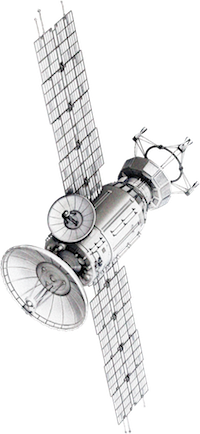
\includegraphics[width=0.8\textwidth]{img-03/satellite}
\end{minipage}

\answers[cols=1]{[Taula: $18:57$; $20:24$; $21:51$; $23:18$; $00:45$; $02:12$, 
		  Expressió general: $t_n = 17:30 + n\cdot 1:27$ on $n$ són el número de voltes completades,
		  Recurrent:  $t_1=18:57$; $t_n=1:27+t_{n-1}$,
		  $t_n = 18:57 + (n-1)\cdot 1:27$ on $n$ són el número de voltes completades,
		  Dividim l'interval 476.5 hores entre el temps d'una volta 1.45 hores: Ha completat 328 voltes a les 13:06.]}

\end{mylist}


\vspace{4cm}

\section{Progressions aritmètiques}

\begin{theorybox}

 \video[ytid=E\_BOmk0n6Eo]{132}{Progressions aritmètiques}

                 Les progressions aritmètiques són successions en què la diferència entre dos termes consecutius (anomenada \textbf{diferència d}) es manté constant. 

      \textbf{Terme General: }  $a_n=\ a_1+d\textrm{·}(n-1)$

 \textbf{Suma dels primers N termes:}  $S_N=N\textrm{·}\frac{(a_1+a_N)}{2}$

\end{theorybox}

 
\begin{mylist}

\exer \spen Assenyala raonadament si la següent successió és una progressió aritmètica: $\{1, 10, 100, 1000, 10000, {\dots}\}$.
\vso
\answers{No és una progressió aritmètica perquè la diferència entre dos termes consecutius no és constant.}

\exer  Calcula els tres primers termes d'una progressió aritmètica sabent que el primer és 1 i la diferència és $-2$.
\vso
\answers{$1,-1,-3,-5,-7,\cdots$}

\begin{resolt}[E]{
		 Calcula el terme 100 \linebreak d'una progressió aritmètica amb diferència 7 i $a_{15} = 165$. 
	}
	Escrivim el terme general de la progressió 
	
	\[a_{15} = 165 = a_1 + 7 \cdot (15 -1)\]
	
	 D'aquí aïllam el valor del primer terme $a_1 = 67$. 
	\vspace{0.25cm}
	
	Ara cercam el terme 100: $a_{100} = 67  + 7 \cdot (100 -1) =760$.
\end{resolt}
 
\exer  Calcula el primer terme d'una progressió aritmètica amb diferència 2 i $a_{30} = 60$. 
\answers{$a_{30}=a_1+2\cdot(30-1)$  $\rightarrow$ $60=a_1+58$, aïllam $a_1=60-58=2$}

\exer  Donada una progressió aritmètica dos dels termes de la qual són: $a_{3} = 4$ i $a_{10} = 18$.

\begin{tasks}(2)
 \task Calcula la seva diferència.
 \task Calcula el seu terme general.
\end{tasks}
\answers[cols=1]{[La diferència és $d=(18-4)/(10-3)=2$, Necessitam el primer terme: $a_1=0$ El terme general és $a_n=0+2\cdot (n-1)$. Efectivament comprovam que $a_{10}=18$]}


\exer  Quin és el terme general d'una progressió aritmètica amb $a_{22} = 45$ i $d = 3$?
\answers{El primer terme és $45=a_1+3\cdot 21$ $\rightarrow$ $a_1 =-18$. El terme general $a_n=-18+3(n-1)$}

\exer  Els costats d'un pentàgon estan en progressió aritmètica de diferència 5. Sabent a més que el seu perímetre és 65, calcula el valor dels costats.
\answers{Recorda que $S=N\cdot \bar x$ on $\bar x$ és el valor mitjà de la progressió aritmètica. $65=5\cdot \bar x$ $\rightarrow$ $x=13$ és el valor d'enmig i els altres les trobam sumant o restant 5: 3; 8; 13; 18 i 23.}

\exer  Calcula els 5 primers termes d'una progressió aritmètica de primer terme 2 i de diferència 3. Representa'ls gràficament. Observa que la seva representació gràfica és un conjunt de punts aïllats que estan sobre una recta.
\answers{2, 5, 8, 11 i 14.}

\exer  Calcula l'expressió general de les progressions aritmètiques:

\begin{tasks}
	\task De diferència $d = 2.5$ i de primer terme 2.
	\task De diferència $d = -2$ i de primer terme 0.
	\task De diferència $d = 1/3$ i de segon terme 5.
	\task  De diferència $d = 4$ i de cinquè terme 1.
\end{tasks}
 \answers[cols=1]{[$a_n=2+2.5(n-1)$, $a_n=0-2(n-1)$, $a_n=\frac{14}{3}+\frac{1}{3}(n-1)$, $a_n=-15+4(n-1)$]}


\exer Quants múltiples de 7 estan compresos entre el 4 i el 893?
\answers{127}

\exer[1]  Suma els 10 primers termes de la progressió aritmètica: $\{-5, 4, 13, 22, 31, 40, {\dots}\}$
\answers{Sumen 355}

\exer[1]  Troba la suma dels 50 primers múltiples de 3.
\answers{Sumen 3825}
	
\begin{comment}
\exer  En una successió aritmètica d'un nombre imparell de termes el central val 12, quant valdrà la suma del primer terme més el darrer terme?

\end{comment}

\exer[1]  L'amo d'un pou contracta a un saurí per conèixer la profunditat a la qual es troba l'aigua i aquest dictamina que a 5 m hi ha aigua en abundància. Demana un pressupost a un contractista, que li diu que el primer metre li costarà 50 euros i per cada mig metre més 6 euros més que pel mig metre anterior. Quant li costarà el pou si es compleixen les prediccions? 
\answers{98 \euro{}}
	
\exer  Antoni s'ha comprat un mòbil, però no pot pagar-ho al comptat. Paga 60 euros cada setmana, però el venedor li puja 5 euros cada setmana en concepte de pagament ajornat. Aconsegueix pagar-ho en 10 setmanes. Quant li va costar? Quant va pagar de més? Quin percentatge suposa aquest recàrrec sobre el preu de venda?
\answers{825, 225, 37.5\%}
	
\exer  Un nedador s'entrena en una piscina de 50 m i vol controlar les pèrdues de velocitat per cansament. Cronometra en cinc dies consecutius els temps que triga a fer 2, 5, 8, 11, 14 llargs. Es demana:

\begin{tasks}
	\task El terme general de la successió $a_n$ que dóna els metres recorreguts en el dia $n$.
	\task  Quants metres haurà nedat en aquests cronometratges?
\end{tasks} 
\answers{[$a_n =100 + 150 (n – 1)$, 100; 250; 400; 550 i 700 metres]}
  

\end{mylist}


%%%%%%%%%%%%%%%%%%%%%%%%%%%%%%%%%%%%%%%%%%%%%%%%%%%%%%%%%%%%%%%%%%%%%%%%%%%%%%%%%%%%%%%%%%%%%%%%%%%%%%%%%%%%%%%%

\section{Progressions geomètriques}

\begin{theorybox}

 \video[ytid=U6kGF1PQEr4]{133}{Progressions geomètriques}

  Les progressions geomètriques són successions en les quals el quocient de dos termes consecutius (anomenat \textbf{raó $r$}) es manté constant. 

  \textbf{Terme general: }  $a_n=\ a_1{\textrm{·}r}^{n-1}$

 \textbf{     Suma dels primers N termes:}  $S_N=\frac{a_1{\textrm{·}(r}^N-1)}{r-1}\ $

 \textbf{     Suma dels infinits termes (si 0$\boldsymbol{<}$r$\boldsymbol{<}$1):} $S_{tots}=\frac{a_1}{1-r}$
\end{theorybox}


\begin{mylist}

\exer \spen Esbrina la raó d'una progressió geomètrica el segon terme de la qual és 27 i el tercer és 3.
\vso
\answers{$r=\frac{3}{27}=\frac{1}{9}$}

\exer \spen  El quart terme d'una progressió geomètrica és $\frac{1}{9}$ i la raó 3. Troba el primer terme.
\vso
\answers{$a_1=\frac{1}{243}$}

\exer  Troba el sisè terme de la següent progressió geomètrica: $\{$$\sqrt{2} $, 2, 2$\sqrt{2} $, 4,{\dots}$\}$
\answers{La raó és $\sqrt{2}$. Els següents termes són: $\{\sqrt{2},2,2\sqrt{2},4,4\sqrt{2},8,8\sqrt{2},16,{\cdots}\}$ }

\end{mylist}

\begin{resolt}[E]{
		D'una progressió geomètrica sabem que $a_1=625$ i $a_4=320$. Troba la raó i el terme cinquè.
	}
	El primer és trobar la raó:
	
	\[ a_4 = a_1 \cdot r^{4-1}  \, \rightarrow \, 320 = 625 \cdot r^3 \, \rightarrow \,  r^3 = 320/625=0,512 \,   \]
	
	La raó és $ r=\sqrt[3]{0,512}=0,8$. Finalment trobam el terme cinquè:
	\[ a_5 = a_1 \cdot r^{5-1}  \, \rightarrow \, a_5 = 625 \cdot (0,8)^4 = 256  \]
	
\end{resolt}

\begin{mylist}
\exer[1]  Donada una progressió geomètrica dos dels termes de la qual són: $a_{3} = -8$ i $a_{5} = -32$. 
\begin{tasks}(2)
	\task   Calcula la seva raó.   \task Calcula el seu terme general.
\end{tasks}
\answers{Raó $-2$, terme general $a_n=(-2)^n$}

\begin{comment}
\exer  Certa classe d'alga, anomenada \textit{clorella}, es reprodueix duplicant la seva quantitat cada dues hores i mitja. Al cap d'altres dues hores i mitja torna a duplicar la seva quantitat, i així successivament. Si es té en el moment inicial un quilo, al cap de dues hores i mitja hi ha dos quilos.


 a) Fes una taula de valors en la qual indiquis per a cada període de reproducció el nombre de quilos de \textit{clorella}.

 b) Indica el terme general.

 c) Al cap de 4 dies, han transcorregut 40 períodes, consideres possible aquest creixement? 
\end{comment}

\exer  Calcula el producte dels 15 primers termes de la progressió: 3, 6, 12, 24, $\cdots$

\answers{Terme general $a_n=3\cdot 2^{n-1}$.\par Terme 15è és $a_{15}=3\cdot 2^{14}=49152$.\par Producte $P_{15}=\sqrt{(3\cdot 49152)^{15}}=5.82\cdot 10^{38}$}

\exer  Un agricultor en la seva granja té 59049 litres d'aigua per donar de beure als animals. Un dia va utilitzar la meitat del contingut, al següent la meitat del que li quedava i així successivament cada dia. Quants litres d'aigua va utilitzar fins al sisè dia?
\answers{$a_1=59049:2=29524.5$. Progressió de raó 1/2 $a_n=29524.5 \cdot (1/2)^{n-1}$.\par El sisè dia consumeix 922.64.\par En total en aquests 6 dies $S_6= \frac{29524.5 \cdot(0.5^6-1)}{0.5-1}=58126.36$ litres. És a dir li queden 922.64 litres.}

\exer[1]  Troba la suma els 15 primers termes d'una progressió geomètrica en la qual $a_{1} = 5$  i $r = \ofrac{1}{2}$.
\answers{Els 15 primers termes sumen $\dfrac{163835}{16384}$}

\exer[1]  Calcula la suma dels infinits termes de la successió: 6, 3, $\frac{3}{2}$, $\frac{3}{4}$, {\dots}
\answers{Els infinits termes sumen 12}

\exer  Tenim a la mà un quadrat d'àrea 1. Tallem les quatre cantonades pels punts mitjans dels costats. El nou quadrat, quina àrea té? Deixem les retallades damunt de la taula. Quina àrea de retallades hi ha sobre la taula? Amb el nou quadrat que tenim a la mà efectuem la mateixa operació de tallar les quatre cantonades i deixar-les sobre la taula, i així successivament. Quina àrea tenen els successius quadrats que tinc a la mà? I les retallades que queden sobre la taula? Troba la suma de les infinites àrees de retallades així obtingudes.
\begin{center}
	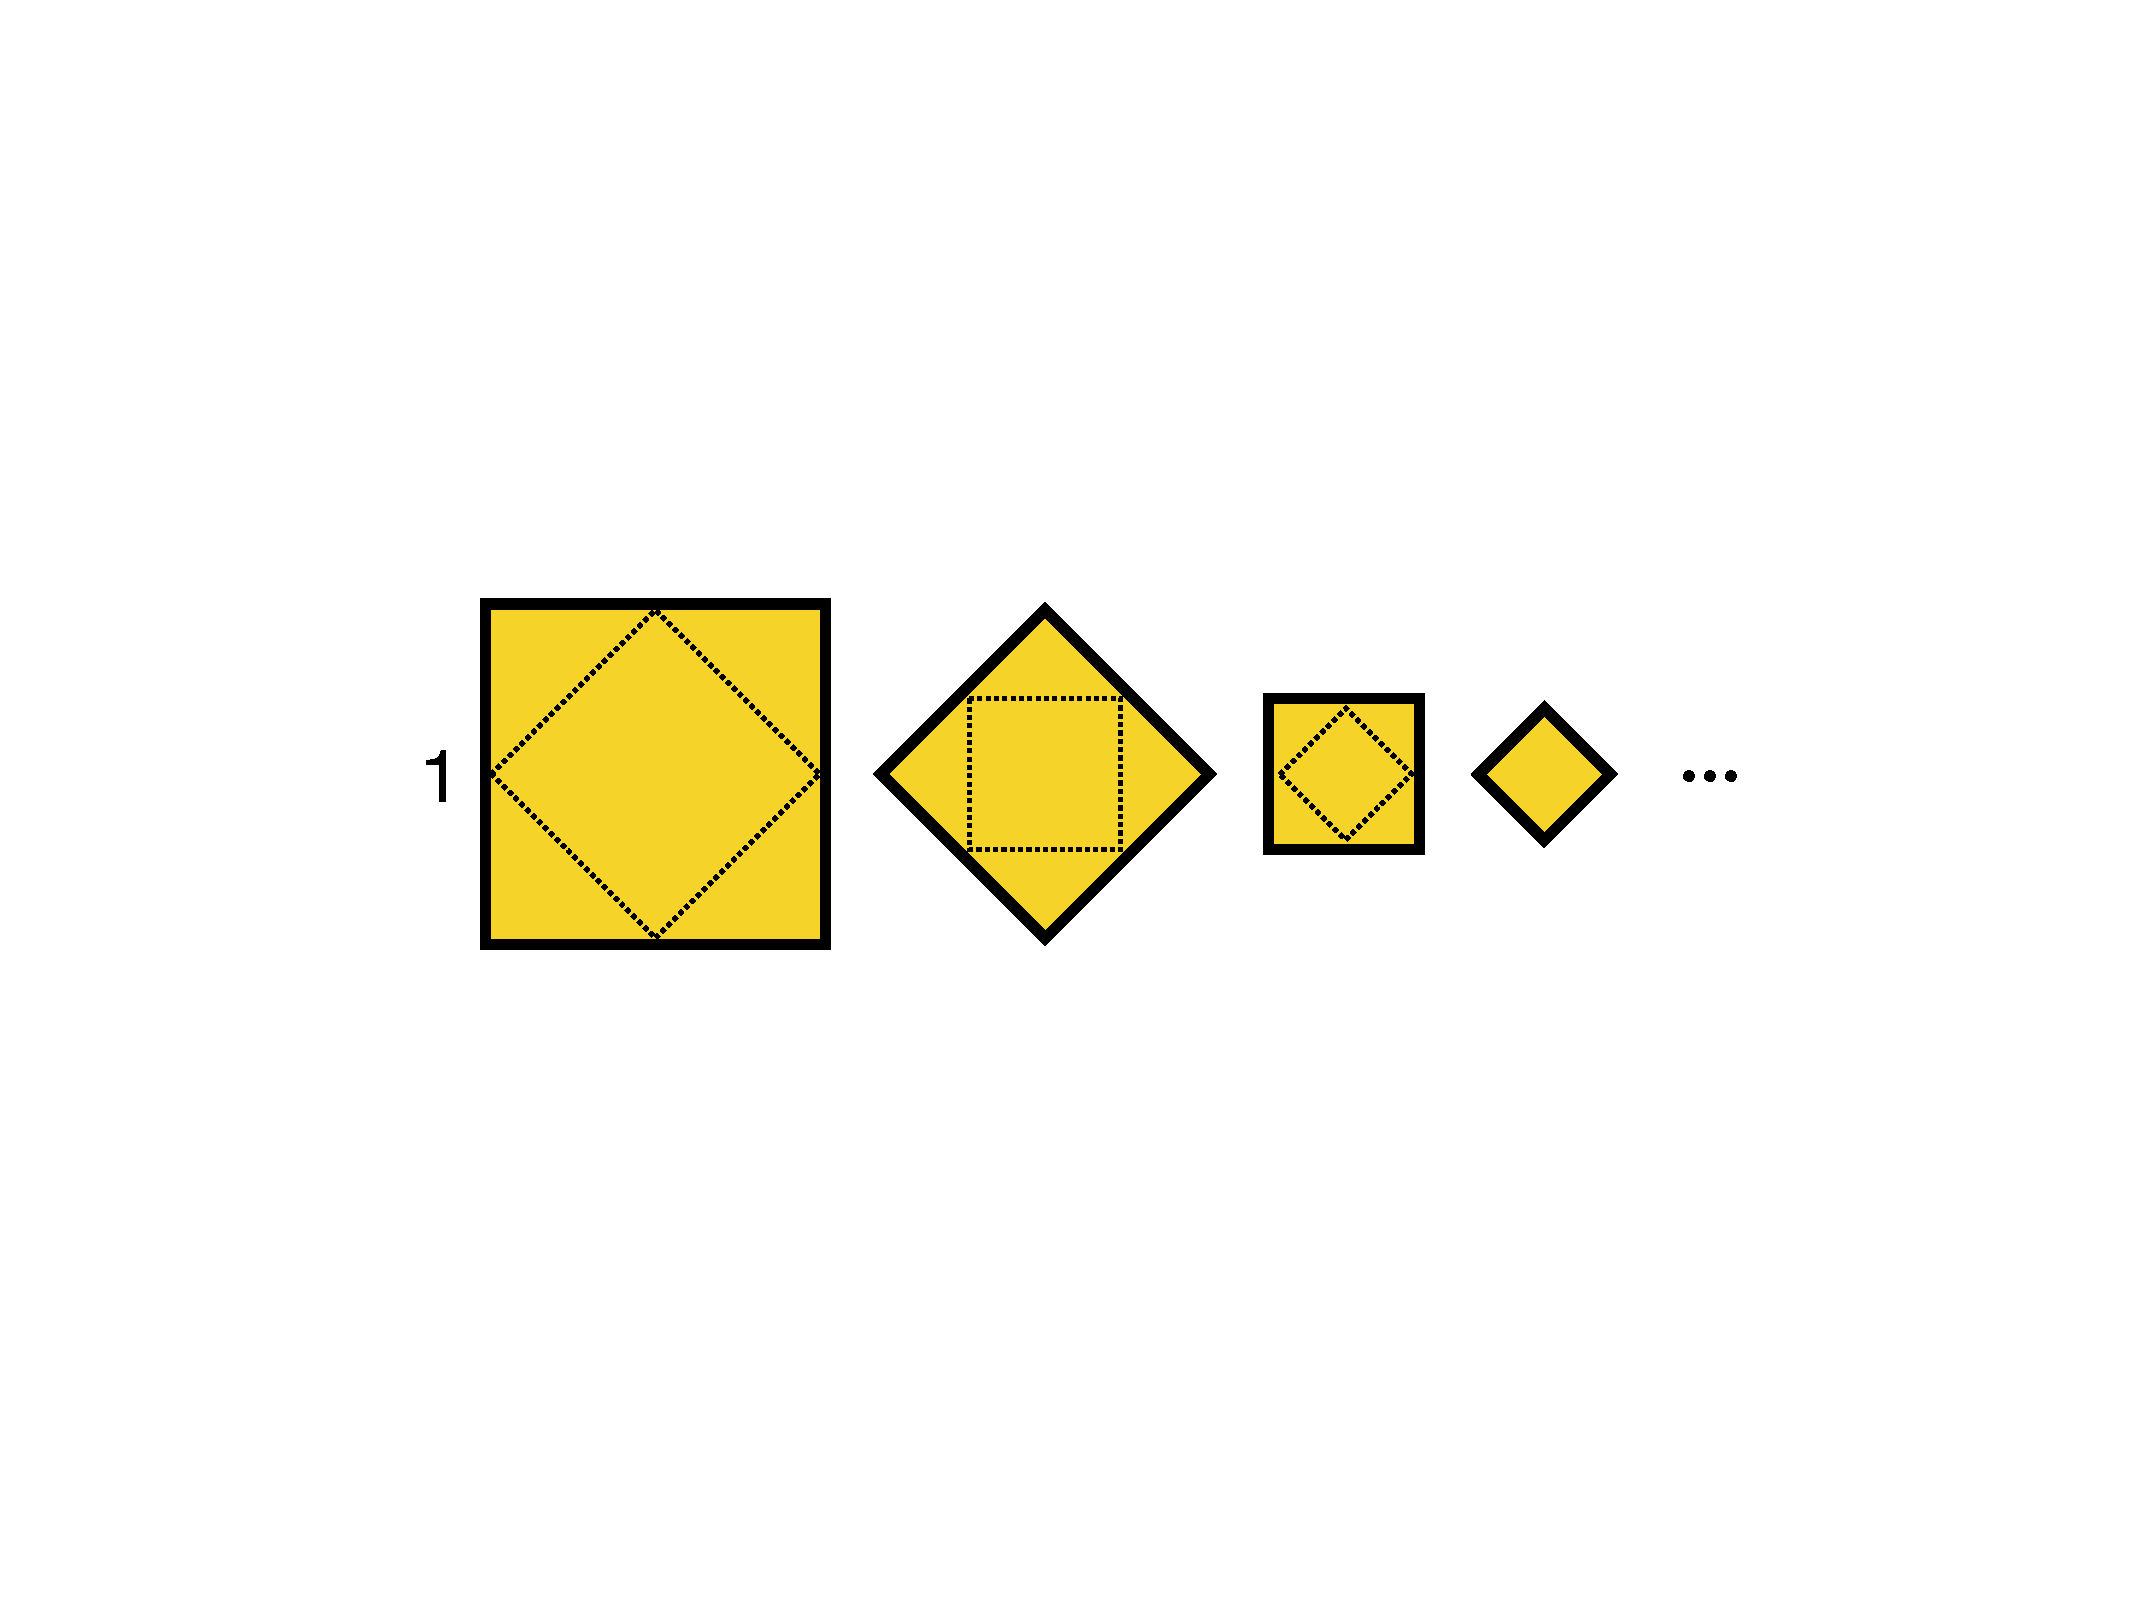
\includegraphics[height=2cm]{img-03/quadrats}
\end{center}
\answers{La successió d'àrees dels quadrats és $1, 1/2, 1/4, 1/8, \cdots$.\par La successió de les retallades és $0, 1/2, 3/4, 7/8, 15/16, \cdots$. \par Veim que la suma de les àrees retallades s'acosta a 1.\par $S_\infy=\frac{0.5}{1-0.5}=1$ }

\begin{comment}
\exer  De nou tenim un quadrat d'àrea 1 a la mà, i ho tallem per les línies de punts com indica la figura. El tros major ho deixem sobre la taula i ens quedem a la mà amb el quadrat, al que tornem a tallar de la mateixa forma. I així successivament. Quina àrea tenen els successius quadrats que tinc a la mà? Creixen o disminueixen? Escriu el terme general de la successió d'àrees que tenim a la mà. I les retallades que queden sobre la taula? Creix l'àrea o disminueix? Anem sumant àrees, calcula la suma d'aquestes àrees si haguéssim fet infinits talls.
\end{comment}

\exer  Calcula la fracció generatriu del número $4,\hat{5}$. Ajuda $4,\hat{5}=4+5\textrm{·}{10}^{-1}+5\textrm{·}{10}^{-2}+\textrm{·}\textrm{·}\textrm{·}$
\answers{$4+5(0.1+0.01+0.001+...)=4+5\frac{0.1}{1-0.1}=4+\frac{5}{9}=\frac{41}{9}$}

\exer  Un empresari acudeix a una entitat financera per informar-se sobre com invertir els 6000 \euro{} de beneficis que ha tingut en un mes. Li plantegen dues opcions.
\begin{tasks}
\task  Mantenir aquest capital durant 5 anys al 3,5 \% anual, 
\task  Rebre el 5 \% del capital durant els dos primers anys i el 3 \% els tres anys restants. 
\end{tasks}
Quina opció li interessa més?
\end{mylist}
\answers{La millor opció és la b) $2\frac{5}{100}\cdot 6000+3\frac{3}{100}\cdot 6000=1140$ euros,\par comparat amb $5\frac{3.5}{100}\cdot 6000= 1050$ euros d'interès.}
\newpage




\begin{activitats}
	
\begin{mylist}
\exer  Calcula el terme 100 d'una progressió aritmètica el primer terme de la qual és 4 i la diferència és 5. 
\answers{$a_{100}=4+5\cdot (100-1)=499$}
 
\exer  El desè terme d'una progressió aritmètica és 45 i la diferència és 4. Troba el primer terme. 
 \answers{$45=a_1+4\cdot (10-1)$ $\,\rightarrow\,$ $a_1=9$}
 
\exer  Sabent que el primer terme d'una progressió aritmètica és 4, la diferència 7 i el terme 88, troba $n$. 
\answers{$88=4+7\cdot(n-1)$ $\,\rightarrow\,$  $n=\frac{88-4}{7}+1=13$}

\exer  Troba el primer terme d'una progressió aritmètica i la diferència, sabent que $a_{3} = 24$ i $a_{10} = 66$. 
\answers{$d=\frac{66-24}{10-3}=6$ $\,\rightarrow\,$  $a_1=24-2\cdot 6=12$}

\exer  El terme sisè d'una progressió aritmètica és 4 i la diferència 1/2. Troba el terme 20. 
\answers{$a_1=1.5$, $a_n=1.5+0.5 (n-1)$. El terme 20 és $a_{20}=1.5+ 0.5 \cdot 19 = 11$}

\exer \hot Calcula els costats d'un triangle rectangle sabent que les seves mesures, expressades en metres, estan en progressió aritmètica de diferència 3. 
\answers{Els costats són  $x-3$, $x$ i $x+3$. Aplicam Pitàgores: $(x+3)^2=(x-3)^2+x^2$, efectuam les identitats notable $x^2-12x=0$, trobam $x=12$. El triangle té costats 9, 12 i 15}

\exer  Calcula la suma dels múltiples de 59 compresos entre 1000 i 2000. 
\answers{Sumen 25075}
\begin{comment}
\exer  El producte de tres termes consecutius d'una progressió aritmètica és 80 i la diferència és 3. Troba aquests termes. 
\end{comment}

\exer  Quants termes cal sumar de la progressió aritmètica 2, 8, 14,... per obtenir com a resultat 1064? 
\answers{S'han de sumar 19 termes}

\exer \hot La suma de \textit{n} nombres naturals consecutius presos a partir d'11 és 1715. Quants termes hem sumat? 
\answers{$\frac{11+11+(n-1)}{2}\cdot n = 1715$. Trobam l'equació $n^2+21n-3430=0$. Hem sumat 49 números}

\exer  Sabent que el cinquè terme d'una progressió aritmètica és 18 i la diferència és 2, troba la suma dels nou primers termes de la successió. 
\answers{Els 9 primers termes sumen 162}

\begin{comment}
\exer  La suma de tres nombres en progressió aritmètica és 33 i el seu producte 1287. Troba aquests nombres. 

\exer  Tres nombres en progressió aritmètica tenen per producte 16640; el més petit val 20. Troba els altres dos. 


\exer  El producte de cinc nombres en progressió aritmètica és 12320 i la seva suma 40. Troba aquests nombres sabent que són enters. 

\exer  Calcula tres nombres sabent que estan en progressió aritmètica, que la seva suma és 18 i que la suma del primer i del segon és igual al tercer disminuït en dues unitats. 

\exer  La suma dels onze primers termes d'una progressió aritmètica és 176 i la diferència dels extrems és 30. Troba els termes de la progressió. 

\exer  La diferència d'una progressió aritmètica és 4. El producte dels quatre primers termes és 585. Troba els termes. 

\exer  En una progressió aritmètica el onzè terme excedeix en 2 unitats al vuitè, i el primer i el novè sumen 6. Calcula la diferència i els termes esmentats. 
\end{comment}
\exer  Sabent que les mesures dels tres angles d'un triangle estan en progressió aritmètica i que un d'ells mesura 100${}^\circ$ , calcula els altres dos. 
\answers{$a_1=100$, $a_2=100-d$, $a_3=100-2d$. La diferència és $40$ i els angles $100^\circ$, $60^\circ$ i $20^\circ$.}

\exer  Troba les dimensions d'un ortòedre sabent que estan en progressió aritmètica, que sumen 78 m i que el volum de l'ortòedre és de 15470 m${}^{3}$. 
\answers{17, 26 i 35}
\begin{comment}
\exer  Els sis angles d'un hexàgon estan en progressió aritmètica. La diferència entre el major i el menor és 60${}^\circ$ . Calcula el valor de cada angle. 
\end{comment}

\exer  Les longituds dels tres costats d'un triangle rectangle estan en progressió aritmètica i sumen 36 metres. Quant mesura cada costat? 
\answers{9, 12 i 15.}

\exer  Un coronel ordena a 5050 soldats que formin un triangle per a una exhibició, de manera que la primera fila tingui un soldat, la segona dues, la tercera tres, etc. Quantes files han d'haver-hi? 
\answers{100 files, perquè $1+2+3+4+\cdots+100=5050$}

\exer  Pel lloguer d'una casa s'acorda pagar 800 euros al mes durant el primer any, i cada any s'augmentarà el lloguer en 50 euros mensuals. Quant es pagarà mensualment al cap de 12 anys? 
\answers{$a_{12}=800+50 (12-1)=1350$ \euro{}.}

\exer  Les edats de quatre germans formen una progressió aritmètica, i la seva suma és 32 anys. El major té 6 anys més que el menor. Troba les edats dels quatre germans. 
\answers{$x$, $x+d$, $x+2d$, $x+3d$. Sabem que $4x+6d=32$ i que $x+3d-x=6$. Llavors $d=2$ i $x=5$. Les edats són $5, 7, 9, 11$ anys.}

\exer  Un esquiador comença la pretemporada d'esquí fent peses en un gimnàs durant una hora. Decideix incrementar l'entrenament 10 minuts cada dia. Quant temps haurà d'entrenar al cap de 15 dies? Quant temps en total haurà dedicat a l'entrenament al llarg de tot un mes de 30 dies? 
\answers{[$a_{15} = 200$ minuts, 6150 minuts en un mes.]}

\exer  En una sala de cinema, la primera fila de butaques dista de la pantalla 86 dm, i la sisena, 134 dm. En quina fila estarà una persona si la seva distància a la pantalla és de 230 dm? 
\answers{$d_n=86+9.6(n-1)$. $230=86+9.6(n-1)$ i aïllam $n$. La fila és la 16}

\exer  Calcula el terme onzè d'una progressió geomètrica el primer terme de la qual és igual a 1 i la raó és 2. 
\answers{$a_{11}=1\cdot 2^{11-1}=2^{10}=1024$}

\exer  En una progressió geomètrica de primer terme 7 i raó 2, un cert terme és 28672. Quin lloc ocupa aquest terme? 
\answers{$28672=7\cdot 2^{n-1}$. Dividim entre 7;\, $4096=2^{n-1}$. Trobam que $n=13$.}

\exer  Sabent que el setè terme d'una progressió geomètrica és 1 i la raó 1/2, troba el primer terme. 
\answers{$1=a_1 \cdot (0.5)^{7-1}$ aïllam $a_1 = \frac{1}{0.5^6}=64$}

\begin{comment}
\exer  El volum d'un ortòedre és de 3375 cm${}^{3}$. Troba la longitud de les seves arestes, sabent que estan en progressió geomètrica i que l'aresta intermèdia mesura 10 cm més que la menor. 


\exer  Troba el producte dels vuit primers termes de la progressió 3, 6, 12, 24,... 
\end{comment}

\exer  Troba la suma dels deu primers termes de la progressió geomètrica 3, 6, 12, 24,... 
\answers{$S_{10}=\frac{3 (2^{10}-1)}{2-1}=3069$}

\exer  Troba la suma dels termes de la progressió il·limitada: 8, 4, 2, 1,... 
\answers{$S_{tots}=\frac{8}{1-0.5}=16$}

\begin{comment}
\exer  Troba tres nombres en progressió geomètrica sabent que la seva suma és 26 i el seu producte 216. 
\end{comment}

\exer  La suma dels set primers termes d'una progressió geomètrica de raó 3 és 7651. Troba els termes primer i setè. 
\answers{$7651=a_1\frac{3^7-1}{3-1}$. Aïllam $a_1=\dfrac{7651}{1093}=7$. El terme 7è $a_7=7\cdot 3^6=5103$.}

\exer \hot  Troba els quatre primers termes d'una progressió geomètrica, sabent que el segon és 20 i la suma dels quatre primers és 425. 
\answers{$r \cdot a_1=20$ i $425=a_1\frac{r^4-1}{r-1}$. Té solució $a_1=5$ i $r=4$ Els termes són: 5, 20, 80 i 320.}

\exer  Les dimensions d'un ortòedre estan en progressió geomètrica. Calcula aquestes dimensions sabent que el seu perímetre és 420 m i el seu volum 8000 m${}^{3}$.
\answers{Les dimensions són 5, 20 i 80}
\begin{comment}
\exer  Divideix el número 221 en tres parts enteres que formen una progressió geomètrica tal que el tercer terme sobrepassa al primer en 136. 
\end{comment}

\exer  La suma de tres nombres en progressió geomètrica és 248 i la diferència entre els extrems 192. Troba aquests nombres. 
\answers{$x+rx+r^2x=248$ i $x(r^2-1)=192$. Els nombres són: 8, 40 i 200} 

\exer  Troba quatre nombres en progressió geomètrica sabent que la suma dels dos primers és 28 i la suma dels dos últims 175. 
 \answers{8, 20, 50 i 125}
 
\exer  Una progressió geomètrica té cinc termes, la raó és igual a la quarta part del primer terme i la suma dels dos primers termes és 24. Troba els cinc termes. 
\answers{$r=x/4$ i $x+rx=24$. Els termes són 8, 16, 32, 64 i 128}

\exer  A una corda de 700 m de longitud se li fan dos talls, de manera que un dels trossos extrems té una longitud de 100 m. Sabent que les longituds dels trossos estan en progressió geomètrica, determina la longitud de cada tros. 
\answers{Els trossos de corda són 100, 200 i 400.}

\exer  Troba la fracció generatriu del nombre decimal 0,737373..., com suma dels termes d'una progressió geomètrica il·limitada.  Ajuda:  $0,737373=73\textrm{·}{100}^{-1}+\ 73\textrm{·}{100}^{-2}+\cdots$
\answers{73/99.}

\exer  Es té una bota de vi que conté 1024 litres. L'1 d'octubre es va buidar la meitat del contingut; l'endemà es va tornar a buidar la meitat del que quedava, i així successivament tots els dies. Quina quantitat de vi es va treure el dia 10 d'octubre? 
\answers{1 litre}

\exer  Donat un quadrat d'1 m de costat, unim dos a dos els punts mitjans dels seus costats; obtenim un nou quadrat, en el qual tornem a efectuar la mateixa operació, i així successivament. Troba la suma de les infinites àrees així obtingudes.
\answers{Les infinites àrees sumen 2 m$^2$} 

\exer  Tres nombres que la seva suma és 36 estan en progressió aritmètica. Troba aquests nombres sabent que si se'ls suma 1, 4 i 43, respectivament, els resultats formen una progressió geomètrica. 
\answers{[PG: 4; 16 i 64, PA: 3; 12 i 21]}

\exer[1] 
\textit{Triangle de Sierpinski}: Anem a construir un fractal. Es parteix d'un triangle equilàter. S'uneixen els punts mitjans dels costats i es formen quatre triangles. S'elimina el triangle central. En cadascun dels altres tres triangles es repeteix el procés. I així successivament. A la figura formada per iteració infinita la hi denomina Triangle de Sierpinski, i és un fractal.
 	\begin{center}
	\includegraphics*[width=0.38\textwidth]{img-03/sierpinski}
\end{center} 

 Imagina que el primer triangle té àrea $A$. Quan apliquem la primera iteració, l'àrea és $(3/4)A$. I en la segona? Escriu la successió de les àrees. És creixent o decreixent? Imagina ara que la longitud de cada costat del triangle inicial és $L$. Escriu la successió de perímetres. És creixent o decreixent? 
 \answers{[$A_n = A \cdot (3/4)^{n-1}$ decreixent, $P_n = 3L \cdot (3/2)^{n-1}$ creixent]}

\end{mylist}
 
\end{activitats}

\pagebreak
\begin{autoaval}{32}

\begin{mylist}

\exer[2]  Quina és la raó de la següent progressió a${}_{ n}$ = 5$\cdot$3\textit{${}^{n}$}${}^{-}$${}^{1}$?
\answers{La raó és 3}

\exer[2]  En la successió $7, 11, 15, 19, 23, \cdots$, quin lloc ocupa el terme 335?
\answers{Posició $n=83$}

\exer[2]  Què val la suma dels deu primers termes de la progressió aritmètica: 7, 13, 19, 31,{\dots}?
 \answers{Sumen 340}
 
\exer[2]  Donada la successió $5, 15, 45, 135, 405, 1215, \cdots$, digues si és una progressió i calcula la seva diferència o raó.
\answers{És una progressió geomètrica. La raó és 3.}

\exer[2]  Calcula el terme general de la successió: $2, 10, 50, 250, 1250, \cdots$.
\answers{Progressió geomètrica $a_{n} = 2 \cdot 5^{n-1}$  }

\exer[2] Quant sumen les potències de 2 compreses entre 2${}^{1}$ i 2${}^{10}$?
\answers{Sumem 2046}
 
\exer[2]  Calcula el terme general de la progressió aritmètica el primer terme de la qual és 1 i la seva diferència 2.
\answers{ $a_{ n} = 2n + 1$ }

\exer[2]  Quin és el valor de la suma: 1 + 3 + 5 + 7 + ... + 999?
\answers{250.000}
 
\exer[2]  Maria està preparant l'examen de selectivitat. Per no deixar tota la matèria per al final ha decidit estudiar cada dia el doble de pàgines que el dia anterior. Si el primer dia va estudiar tres pàgines, quantes haurà estudiat al cap de 7 dies? Quantes pàgines haurà estudiat en total?
\answers{192 pàgines dia 7; 381 pàgines en total}
 
\exer[2]  A n'en Bernat li han tocat 6000 \euro{} en la loteria i decideix dipositar-los al banc a un tipus d'interès compost del 4 \%. Quants diners tindrà al cap de 5 anys?
\answers{$6000\cdot 1,04^5 = 7299,92$ \euro{}}

\end{mylist}

\end{autoaval}

\vsoo

\begin{blueshaded}
	
	La successió de \textbf{Fibonacci} comença amb dos uns i després cada terme s'obté de sumar el dos anteriors. Aquests són els primers termes:
	$
	 1, 1, 2, 3, 5, 8, 13, 21, 34, 55, 89, \cdots
	$
	
	Aquesta successió apareix en molts de casos en la naturalesa, especialment en estructures espirals com ara els caragols, el nombre de pètals de les margalides, els girasols, les pinyes, les galàxies, etc.
	
	\vspace{0.25cm}
	
	\begin{center}
		
\includegraphics[height=3cm]{img-03/espiral.png}
		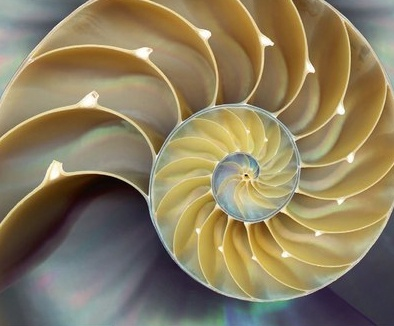
\includegraphics[height=3cm]{img-03/nautilus2.jpg}
	\end{center}

Cerca més informació sobre aquesta successió i  la seva relació amb el nombre auri.
	
	\begin{comment}
	Aquesta successió té una propietat curiosa. Si dividim dos termes consecutius trobam la successió:
	
	\[1, 2, 1.5, 1.6, 1.625, 1.6154, 1.619, 1.617, \cdots\]
	
	Resulta que aquesta successió s'acosta a un nombre que és tan important que se li va donar un nom (\textbf{el nombre auri}) $\Phi = \frac{1+\sqrt{5}}{2} = 1.618034 \cdots$
	\end{comment}
\end{blueshaded}

\newpage
\resum 

\begin{longtable}{|p{0.5\textwidth}|p{0.4\textwidth}|} \hline 
 \rowcolor{lightgray} \multicolumn{2}{|c|}{\textbf{ PROGRESSIÓ ARITMÈTICA}} \\ \hline
 És una successió de nombres reals en la qual la diferència entre dos termes consecutius de la successió és constant. Aquesta constant s'anomena \textbf{diferència} de la progressió i se sol denotar amb la lletra \textit{d}. & 2, 5, 8, 11, 14, 17, {\dots} \\ \hline 
 \rowcolor{lightgray} \multicolumn{2}{|p{0.5\textwidth}|}{\textbf{Terme general}} \\ \hline
\textit{a}${}_{ n}$ = \textit{a${}_{ }$}${}_{1}$ + \textit{d}·(\textit{n $-$ 1}) essent \textit{a}${}_{ 1}$ el primer terme & \[a_n = 2 + 3n \] \\ \hline 
\rowcolor{lightgray} \multicolumn{2}{|p{0.5\textwidth}|}{\textbf{Suma dels $n$ primers termes}} \\ \hline
 \[S_{n} =\frac{n\cdot (a_{1} +a_{n} )}{2} \] & \[S_{8} =\frac{8\cdot (2+(2+3\cdot 8))}{2}  =\] \[ = 4 \cdot (4 + 24) = 4 \cdot 28 = 112 \] \\ \hline \hline 
 \rowcolor{lightgray} \multicolumn{2}{|c|}{\textbf{PROGRESSIÓ GEOMÈTRICA}} \\ \hline
  És una successió de nombres reals en la qual el quocient entre cada terme i l'anterior és constant. A aquesta constant es denomina \textbf{raó} de la progressió i se sol denotar amb la lletra \textit{r}.\newline És a dir, $\frac{a_{i+1} }{a_{i} } =r$ sent \textit{i} un nombre natural. & \[ 3, 6, 12, 24, {\dots} \] \newline \[ 1, 1/2, 1/4, 1/8{\dots}\] \\ \hline 
  \rowcolor{lightgray} \multicolumn{2}{|p{0.5\textwidth}|}{\textbf{Terme general}} \\ \hline
 \[ a_n = a_1 \cdot r^{n-1}\] essent \textit{a${}_{ }$${}_{1}$} el primer terme de la successió & \[ a_n= 3 \cdot 2^{n-1} \]
 
 \[a_n = 1 \cdot (1/2)^{n} \] \\ \hline 
 \rowcolor{lightgray} \multicolumn{2}{|p{0.5\textwidth}|}{\textbf{Suma dels termes  }} \\ \hline
- Per a un \underbar{nombre $n$} de termes: \newline \[ S_n =\frac{r\cdot a_{n} -a_{1} }{r-1}  = \frac{a_{1} (r^{n} -1)}{r-1} \] \newline - Per a  $r<1$, i una \underbar{quantitat il·limitada} de termes:\[ S_{tots}=\frac{a_{1} }{1-r} \] & \[S_{8} = \frac{3(2^{8} -1)}{2-1}  = 3(256 - 1) =   765\] \newline \[S_{tots}=\frac{1}{1-\frac{1}{2} } = 2 \] \\ \hline 
\rowcolor{lightgray} \multicolumn{2}{|p{0.5\textwidth}|}{\textbf{Producte dels $n$ primers termes}} \\ \hline
 \textit{P${}_{n}$} = $\pm \sqrt{\left(a_{1} \cdot a_{n} \right)^{n} } $ = $\pm a_{1} \cdot r^{\ofrac{n-1}{2} } $  & \textit{P}${}_{9}$ = + $\sqrt{(3\cdot (3\cdot 2^{8} ))^{9} } $=(3 $\cdot$ 2${}^{4}$)${}^{9}$\newline  \\ \hline 
\end{longtable}


\begin{extrapage}
	
\setcounter{myenumi}{0}
\heading{FITXA 1: EXERCICIS DE SUCCESSIONS}
\vso

\begin{mylist}
	
	\item Escriu els tres primers termes de les successions
	\begin{tasks}(2)
		\task $a_n = (n-1)^3$
		\task $b_n = n + \frac{3}{n+1}$
		\task $c_n = 3 + 5(n-1)$
		\task $d_n = 3 \cdot \left( \frac{1}{2} \right)^n$
		\task $e_n = (n-1)(n-2)$
		\task $f_n = n^2 - n$
	\end{tasks}
	
	\item Calcula el terme que ocupa el lloc desè de les successions següents:
	\begin{tasks}(3)
		\task $a_n = 3n-1$
		\task $b_n = \frac{n^2+1}{2}$
		\task $c_n = (-1)^n + \frac{1}{n}$
		\task $d_n=\frac{1}{2}+\frac{(-1)^{n+1}}{10}$
		\task $e_n = n (n-1)$
		\task $f_n = \frac{n}{3} + \frac{3}{n}$
	\end{tasks}
	
	\item Forma una successió recurrent amb aquestes dades. Escriure-ne només els 6 primers termes.
	
	\qquad $j_1=2$  \qquad $j_2=3$  \qquad $j_n=j_{n-1} - j_{n-2}$  
 	
	\item Escriu els quatre primers termes de la successió següent: $a_1=\frac{1}{3}$ i $a_n = 2 a_{n-1}+3$.
	
	\item Troba el terme general de cada una de les successions. Calcula el terme 100è.
	\begin{tasks}(2)
		\task 12, 14, 16, 18, $\cdots$
		\task $\frac{1}{2}$, $\frac{2}{3}$, $\frac{3}{4}$, $\frac{4}{5}$, $\cdots$
		\task $-1$ 2, $-3$, 4, $\cdots$
		\task 1, 3, 9, 27, $\cdots$
	\end{tasks}
	
	\item Afegeix un terme nou i escriu la relació de recurrència de la successió següent: 
	$1, 2, 3, 6, 11, 20, \cdots$  (\textit{Pista: relaciona cada terme amb els tres anteriors.})
	
		\item Calcula $a_1$, $a_2$ i $a_{10}$ de cadascuna de les successions següents:
	\begin{center}
		\renewcommand{\arraystretch}{1.5}
		\begin{longtable}{|p{0.03\textwidth}|p{0.3\textwidth}|p{0.1\textwidth}|p{0.1\textwidth}|p{0.1\textwidth}|} \hline 
		\rowcolor{lightgray}	& $\mathbf{a_n}$ & $a_1$ & $a_2$ & $a_{10}$ \\ \hline
		\cellcolor{lightgray}	a) & $a_n = 2n-1$ &  &  &  \\ \hline
		\cellcolor{lightgray}	b) & $a_n = \frac{4n-3}{2}$ & & & \\ \hline
		\cellcolor{lightgray}	c) & $a_n = n^2 -3n+5$ & & & \\  \hline
		\cellcolor{lightgray}	d) & $a_n = 2^{n-1}$ & & & \\  \hline
		\cellcolor{lightgray}	e) & $a_n= (-3)^n$ & & & \\  \hline
		\end{longtable}	
	\end{center}	
\end{mylist}

\end{extrapage}	

\newpage

\begin{extrapage}
	
\setcounter{myenumi}{0}

\heading{FITXA 2: EXERCICIS DE PROGRESSIONS}


\begin{center}
	\textbf{RECORDA:} 
	\textbf{Aritmètica}: $a_n=a_1+d\cdot (n-1)$ \qquad \textbf{Geomètrica}: $a_n= a_1 \cdot r^{n-1}$
\end{center}

\begin{mylist}
	
	\item Digues si són Successió, Progressió aritmètica o Progressió geomètrica. Escriu dos termes més en cada cas. En cas que sigui una progressió digues què val la seva diferència $d$ o la raó $r$.
	
	\begin{longtable}{|p{0.25\textwidth}|p{0.25\textwidth}|p{0.22\textwidth}|p{0.22\textwidth}|} \hline 
	\rowcolor{lightgray}	& \textbf{Succ., PA o PG?} & $\mathbf{a_5}$ & $\mathbf{a_6}$ \\ \hline 
		a) 100, 80, 64, 51.2, ... & & & \\ \hline 
		b) 1, 4, 9, 16, ... & & & \\ \hline 
		c) 1.2, 0.8, 0.4, 0, ...& & & \\ \hline 
		d) 16, 24, 36, 54, ... & & & \\ \hline 
	\end{longtable}

	
	\item Escriu el terme general de les \underline{progressions} de l'exercici anterior.
 	
	\item Calcula el terme 31 de les progressions següents:
	\begin{longtable}{|p{0.33\textwidth}|p{0.31\textwidth}|p{0.31\textwidth}|} \hline 
	\rowcolor{lightgray} & $\mathbf{a_n}$ & $\mathbf{a_{31}}$ \\ \hline 
	a) 3, 6, 12, 24, ... & &  \\ \hline 
	b) 19, 26, 33, 40, ... & &  \\ \hline 
	c) 90, --30, 10, --10/3, ...& &  \\ \hline 
	d) 5, 7, 9, 11, 13, ... & &  \\ \hline 
	e) 80, 8, 0.8, 0.08, ... & &  \\ \hline 
	\end{longtable}	 
	
	\item En una progressió geomètrica sabem que $a_{10}=50$ i $a_{11}=60$. Calcula el primer terme.
	  
	\item El tercer terme d'una progressió geomètrica és 12 i la raó 5; calcula el terme desè.
	
	\item La dosi d'un medicament és de 100 mg el primer dia i 0.5 mg menys cadacun dels dies següents. El tractament dura 120 dies. Quina quantitat de medicament ha près en total el malalt?
	
	\item Un tipus de bacteri es reprodueix per bipartició, és a dir, es duplica cada quart d'hora. Si inicialment hi havia 10 bacteris, quants n'hi haurà passades 6 hores?
	
	\item Calcula les següents sumes:
	\begin{tasks}(2)
		\task 1 + 3 + 5 + $\cdots$ + 999
		\task 3 + 5 + 8 + $\cdots$ + 253
		\task 0.2 + 0.4 + 0.8 + $\cdots$ + 102.4
	\end{tasks}


	\item He decidit estalviar diners, 2 euros per començar i 20 cèntims cada dia. Em demano quants de diners tindré estalviats al cap d'un mes (de 30 dies)?
	
	
	\item La meva cosina ha tornat encantada de les vacances. Ha compartit amb 3 amics les seves fotos en la xarxa social. Cadascun d'ells, al seu torn, les comparteix amb 3 amics més, i així successivament. Quantes persones podran veure les fotos de les vacances de la meva cosina si s'han compartit fins el grau 10è d'amistat?
	
	
\end{mylist}


\end{extrapage}